%!TEX root = ../thesis.tex
% ******************************* Thesis Appendix A ****************************
\chapter{Appendix} 
\ifpdf
\graphicspath{{Chapter3/Figs/Raster/}{Chapter3/Figs/PDF/}{Chapter3/Figs/}}
\else
\graphicspath{{Chapter3/Figs/Vector/}{Chapter3/Figs/}}
\fi
Here we present additional results for different features sets than the ones presented in Chapter \ref{chap:results}, so as to complete and complement the discussion without burdening the reader with long, difficult to read tables and figures.

The PCoA sets presented here were computed using the Bray-Curtis distance measure; their only difference with the ones presented in the Results \& Discussion Chapter is that only some of the axes where used for classification. In particular, the first axes to describe 99\% and 90\% of the variance were used. Also, the configuration of a 20-dimensional NMDS ordination was used as a feature set. The procedure was run for 10000 steps and did not converge, so it does not represent the best 20-dimensional NMDS configuration.


The results for maximum similarity are presented in tables \ref{table:lrsimilarityappendix} for Logistic regression and \ref{table:rfrsimilarityappendix} for Random Forest. As with the other feature sets, Logistic regression is outperforming Random Forest (except for NMDS). Both methods are above the baseline.
%SIMILARITY
%SIM LOG 
\begin{table}[h]
	\centering
	\begin{tabular}{l c  c c}
		\toprule
		&\multicolumn{2}{c}{Confusion Matrix} & Accuracy\\
		Features used & Predicted Black&Predicted White&\\
		\midrule
		\multirow{2}{*}{PCoA 99\%} &16 &5&\multirow{2}{*}{95.12\%}\\
		&	 3&140&\\
		\cmidrule{2-3}
		\multirow{2}{*}{PCoA 90\%} &16 &5&\multirow{2}{*}{95.12\%}\\
		&	 3&140&\\
		\cmidrule{2-3}
		\multirow{2}{*}{PCoA CSS 99\%} &16 &5&\multirow{2}{*}{96.34\%}\\
		&	 1&142&\\
		\cmidrule{2-3}
		\multirow{2}{*}{PCoA CSS 90\%} &16 &5&\multirow{2}{*}{95.73\%}\\
		&	 2&141&\\
		\cmidrule{2-3}
		\multirow{2}{*}{NMDS}&13 &8&\multirow{2}{*}{90.24\%}\\
		&	 8&135&\\
				\cmidrule{2-3}
		\multirow{2}{*}{PCA}&4 &17&\multirow{2}{*}{88.41\%}\\
		&	 2&141&\\
		\bottomrule
	\end{tabular}
	\caption{Results from maximising similarity using Logistic Regression. The percentages indicate the total variance the axes of PCoA explain.}
	\label{table:lrsimilarityappendix}
\end{table}

%RFR SIMILARITY
\begin{table}[h]
	\centering
	\begin{tabular}{l c  c c}
		\toprule
		&\multicolumn{2}{c}{Confusion Matrix} & Accuracy\\
		Features used & Predicted Black&Predicted White&\\
		\midrule
		\multirow{2}{*}{PCoA 99\%} &4 &17&\multirow{2}{*}{86.59\%}\\
		&	 5&138&\\
		\cmidrule{2-3}
		\multirow{2}{*}{PCoA 90\%} &9 &12&\multirow{2}{*}{90.24\%}\\
		&	 4&139&\\
		\cmidrule{2-3}
		\multirow{2}{*}{PCoA CSS 99\%} &10 &11&\multirow{2}{*}{93.29\%}\\
		&	 0&143&\\
		\cmidrule{2-3}
		\multirow{2}{*}{PCoA CSS 90\%} &12 &9&\multirow{2}{*}{94.51\%}\\
		&	 0&143&\\
		\cmidrule{2-3}
		\multirow{2}{*}{NMDS}&10 &11&\multirow{2}{*}{92.07\%}\\
		&	 2&141&\\
						\cmidrule{2-3}
		\multirow{2}{*}{PCA}&2 &19&\multirow{2}{*}{88.41\%}\\
		&	 0&143&\\
		\bottomrule
	\end{tabular}
	\caption{Results from maximising similarity using Random Forest. The percentages indicate the total variance the axes of PCoA explain.}
	\label{table:rfrsimilarityappendix}
\end{table}
%PIE SIMILARITY






%DISSIMILARITY
The results for maximum dissimilarity are presented in tables \ref{table:lrdissimilarityappendix} for Logistic regression and \ref{table:rfrdissimilarityappendix} for Random Forest. Unlike the other feature sets in the same setting, Logistic regression is outperforming Random Forest (except for NMDS). Both methods are above the baseline. It is interesting to note that the sets PCoA 90\% and PCoA CSS 99\% produce a better accuracy for Logistic regression than its best set in Chapter \ref{chap:results}. 
%LOG DISSIM
\begin{table}[h]
	\centering
	\begin{tabular}{l c  c c}
		\toprule
		&\multicolumn{2}{c}{Confusion Matrix} & Accuracy\\
		Features used & Predicted Black&Predicted White&\\
		\midrule
		\multirow{2}{*}{PCoA 99\%} &7 &14&\multirow{2}{*}{86.59\%\%}\\
		&	 8&135&\\
		\cmidrule{2-3}
		\multirow{2}{*}{PCoA 90\%} &7 &14&\multirow{2}{*}{88.41\%}\\
		&	 5&138&\\
		\cmidrule{2-3}
		\multirow{2}{*}{PCoA CSS 99\%} &8 &13&\multirow{2}{*}{89.02\%}\\
		&	 5&138&\\
		\cmidrule{2-3}
		\multirow{2}{*}{PCoA CSS 90\%} &8 &13&\multirow{2}{*}{85.37\%}\\
		&	11&132&\\
		\cmidrule{2-3}
		\multirow{2}{*}{NMDS}&3 &18&\multirow{2}{*}{82.93\%}\\
		&	 10&133&\\
						\cmidrule{2-3}
		\multirow{2}{*}{PCA}&0 &21&\multirow{2}{*}{87.20\%}\\
		&	 0&143&\\
		\bottomrule
	\end{tabular}
	\caption{Results from maximising dissimilarity using Logistic Regression. The percentages indicate the total variance the axes of PCoA explain.}
	\label{table:lrdissimilarityappendix}
\end{table}

%RFR DISSIM
\begin{table}[h]
	\centering
	\begin{tabular}{l c  c c}
		\toprule
		&\multicolumn{2}{c}{Confusion Matrix} & Accuracy\\
		Features used & Predicted Black&Predicted White&\\
		\midrule
		\multirow{2}{*}{PCoA 99\%} &0 &21&\multirow{2}{*}{84.76\%}\\
		&	4&139&\\
		\cmidrule{2-3}
		\multirow{2}{*}{PCoA 90\%}  &0 &21&\multirow{2}{*}{84.76\%}\\
		&	4&139&\\
		\cmidrule{2-3}
		\multirow{2}{*}{PCoA CSS 99\%}  &0 &21&\multirow{2}{*}{84.76\%}\\
		&	4&139&\\
		\cmidrule{2-3}
		\multirow{2}{*}{PCoA CSS 90\%} &0 &21&\multirow{2}{*}{84.15\%}\\
		&	5&138&\\
		\cmidrule{2-3}
		\multirow{2}{*}{NMDS}&1 &20&\multirow{2}{*}{86.59\%}\\
		&	 2&141&\\
						\cmidrule{2-3}
		\multirow{2}{*}{PCA}&0 &21&\multirow{2}{*}{81.71\%}\\
		&	 9&134&\\
		\bottomrule
	\end{tabular}
	\caption{Results from maximising dissimilarity using Random Forest. The percentages indicate the total variance the axes of PCoA explain.}
	\label{table:rfrdissimilarityappendix}
\end{table}
%PIE DISSIM

We used the feature importance method of Random Forest to determine which taxonomic Orders contribute the most to the predictive power of the classifier. Figure \ref{fig:dispieappendix} shows the mean and sum aggregation for the OTU and OTU MIN CSS feature sets in the maximum similarity setting. Figure \ref{fig:simpieappendix} for the maximum dissimilarity.

\begin{figure}[h]
	\centering
	\begin{subfigure}{0.45\textwidth}
		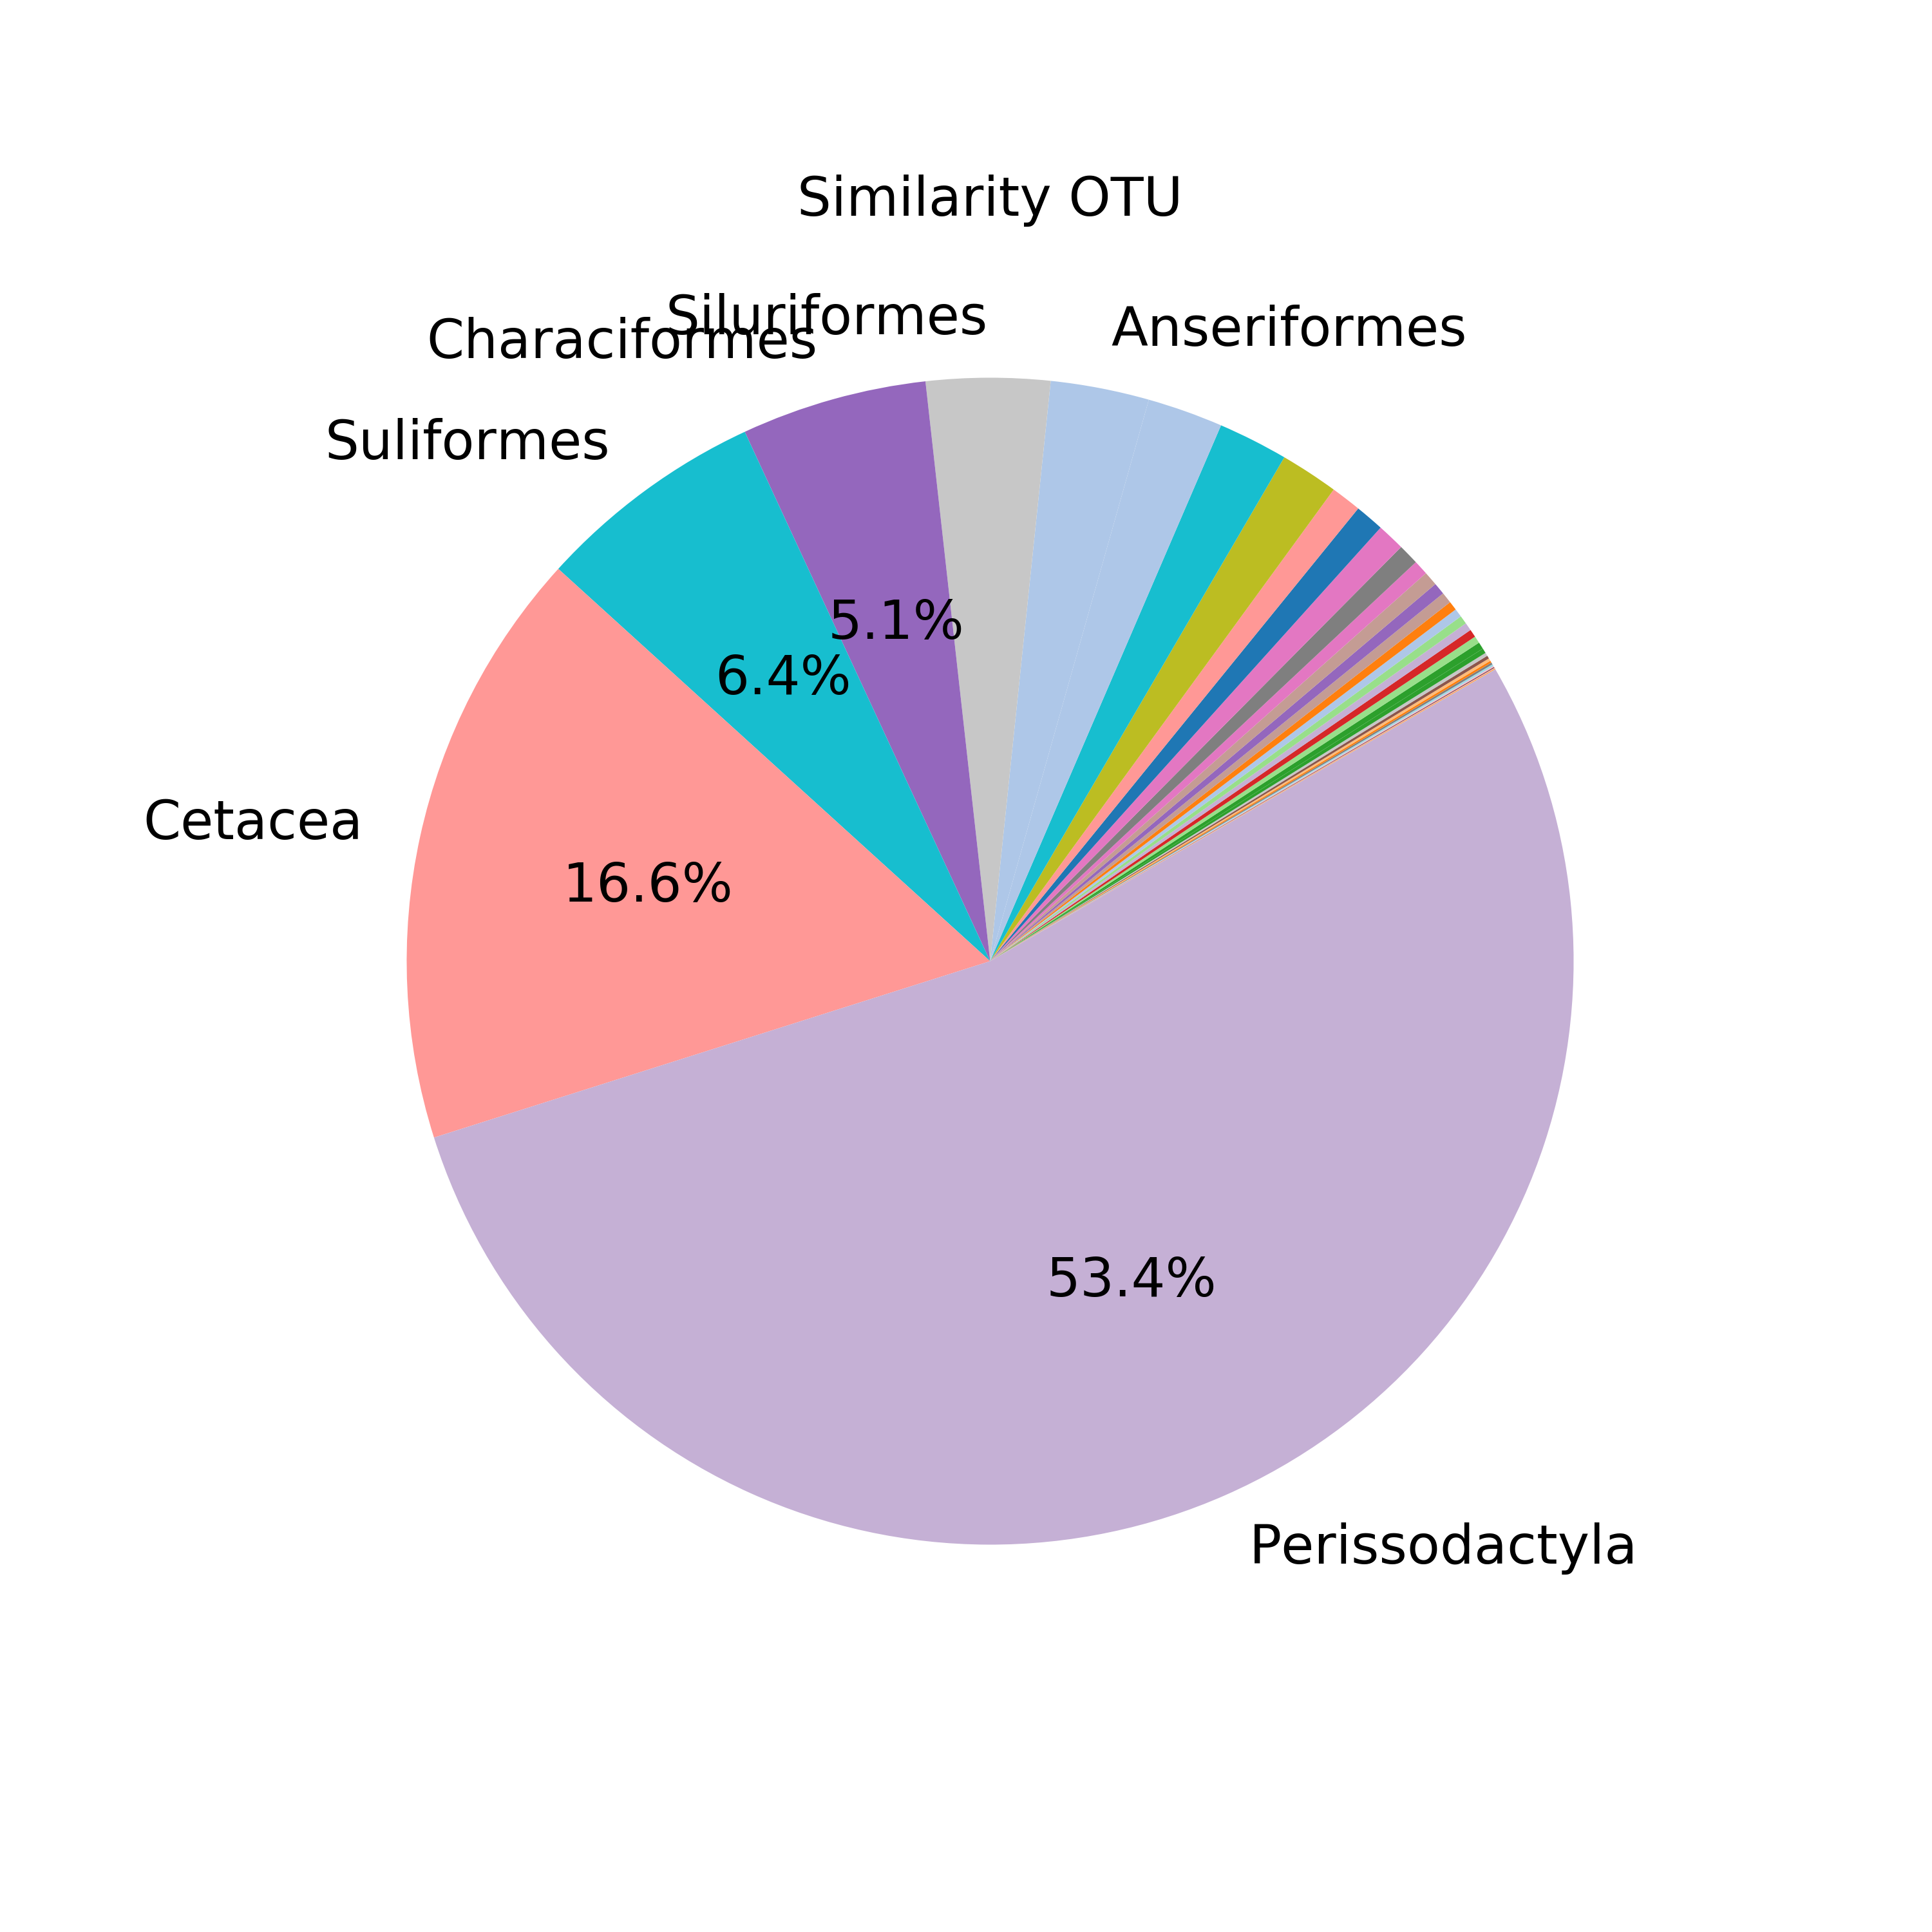
\includegraphics[width=\textwidth]{rfr_sim_mean_pieOTU}
		\caption{}
		\label{fig:simotumean}
	\end{subfigure}
	\begin{subfigure}{0.45\textwidth}
		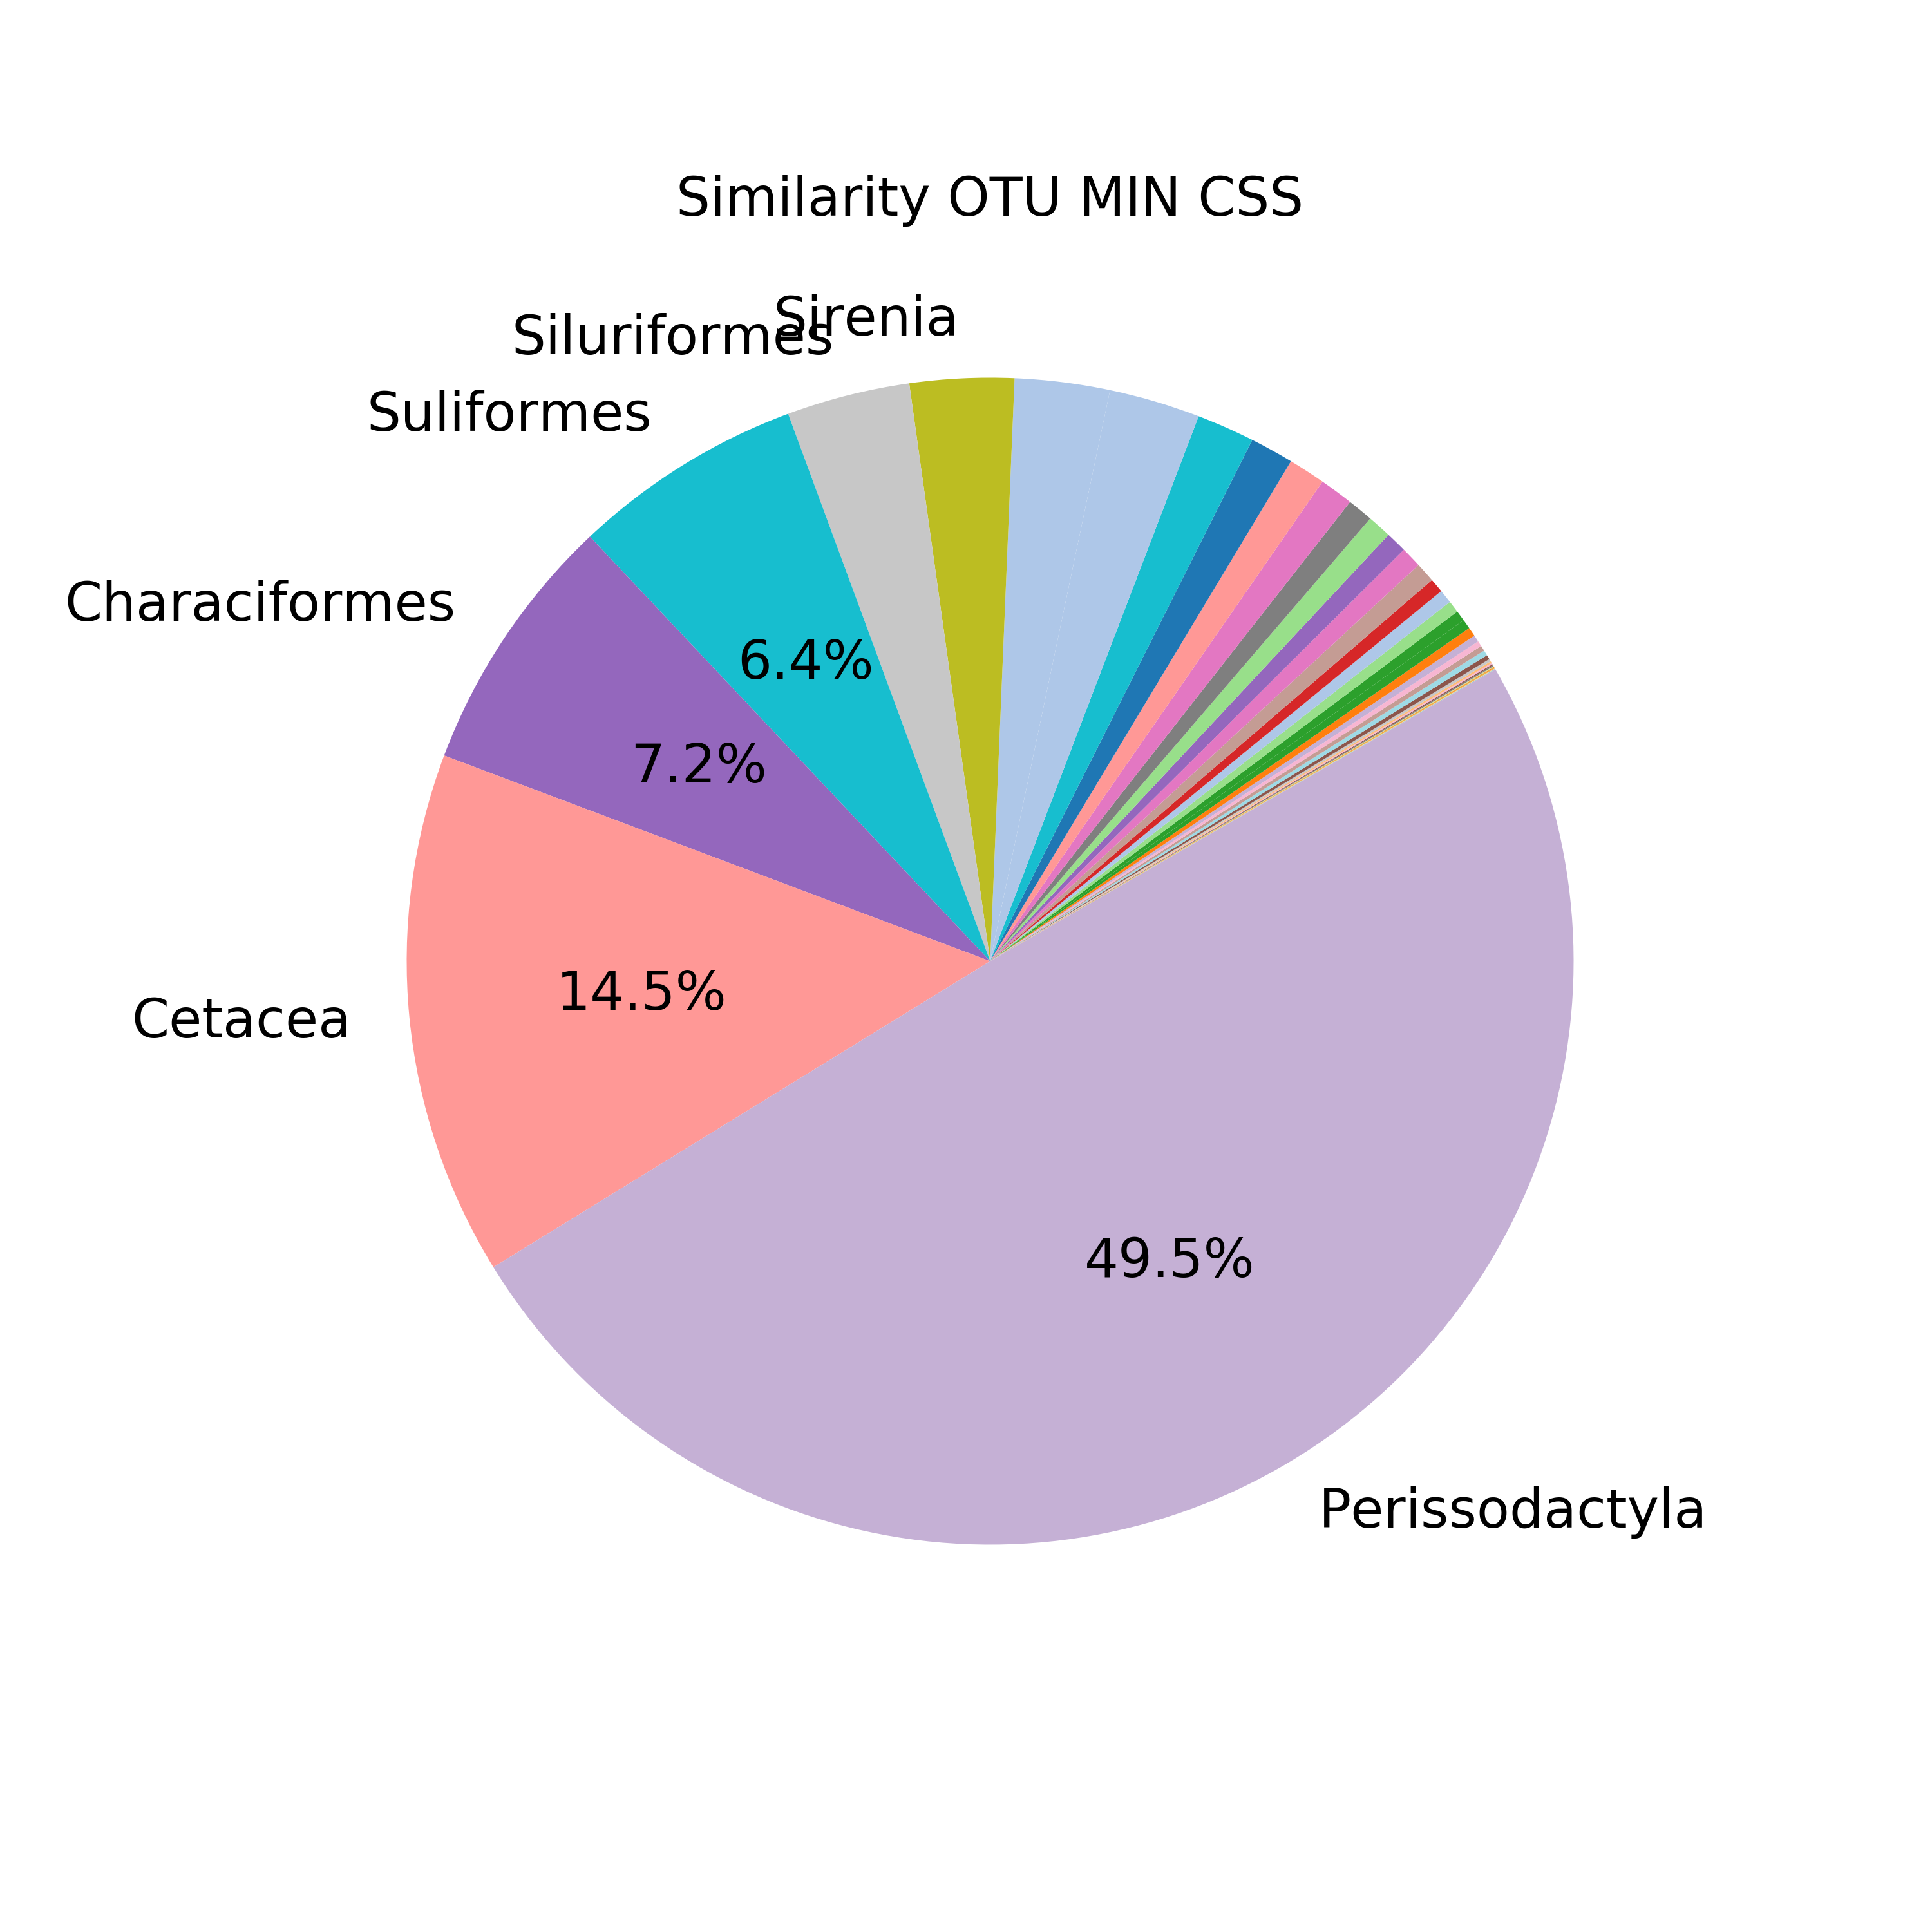
\includegraphics[width=\textwidth]{rfr_sim_mean_pieOTU MIN CSS}
		\caption{}
		\label{fig:simotumincssmean}
	\end{subfigure}\\
	\begin{subfigure}{0.45\textwidth}
		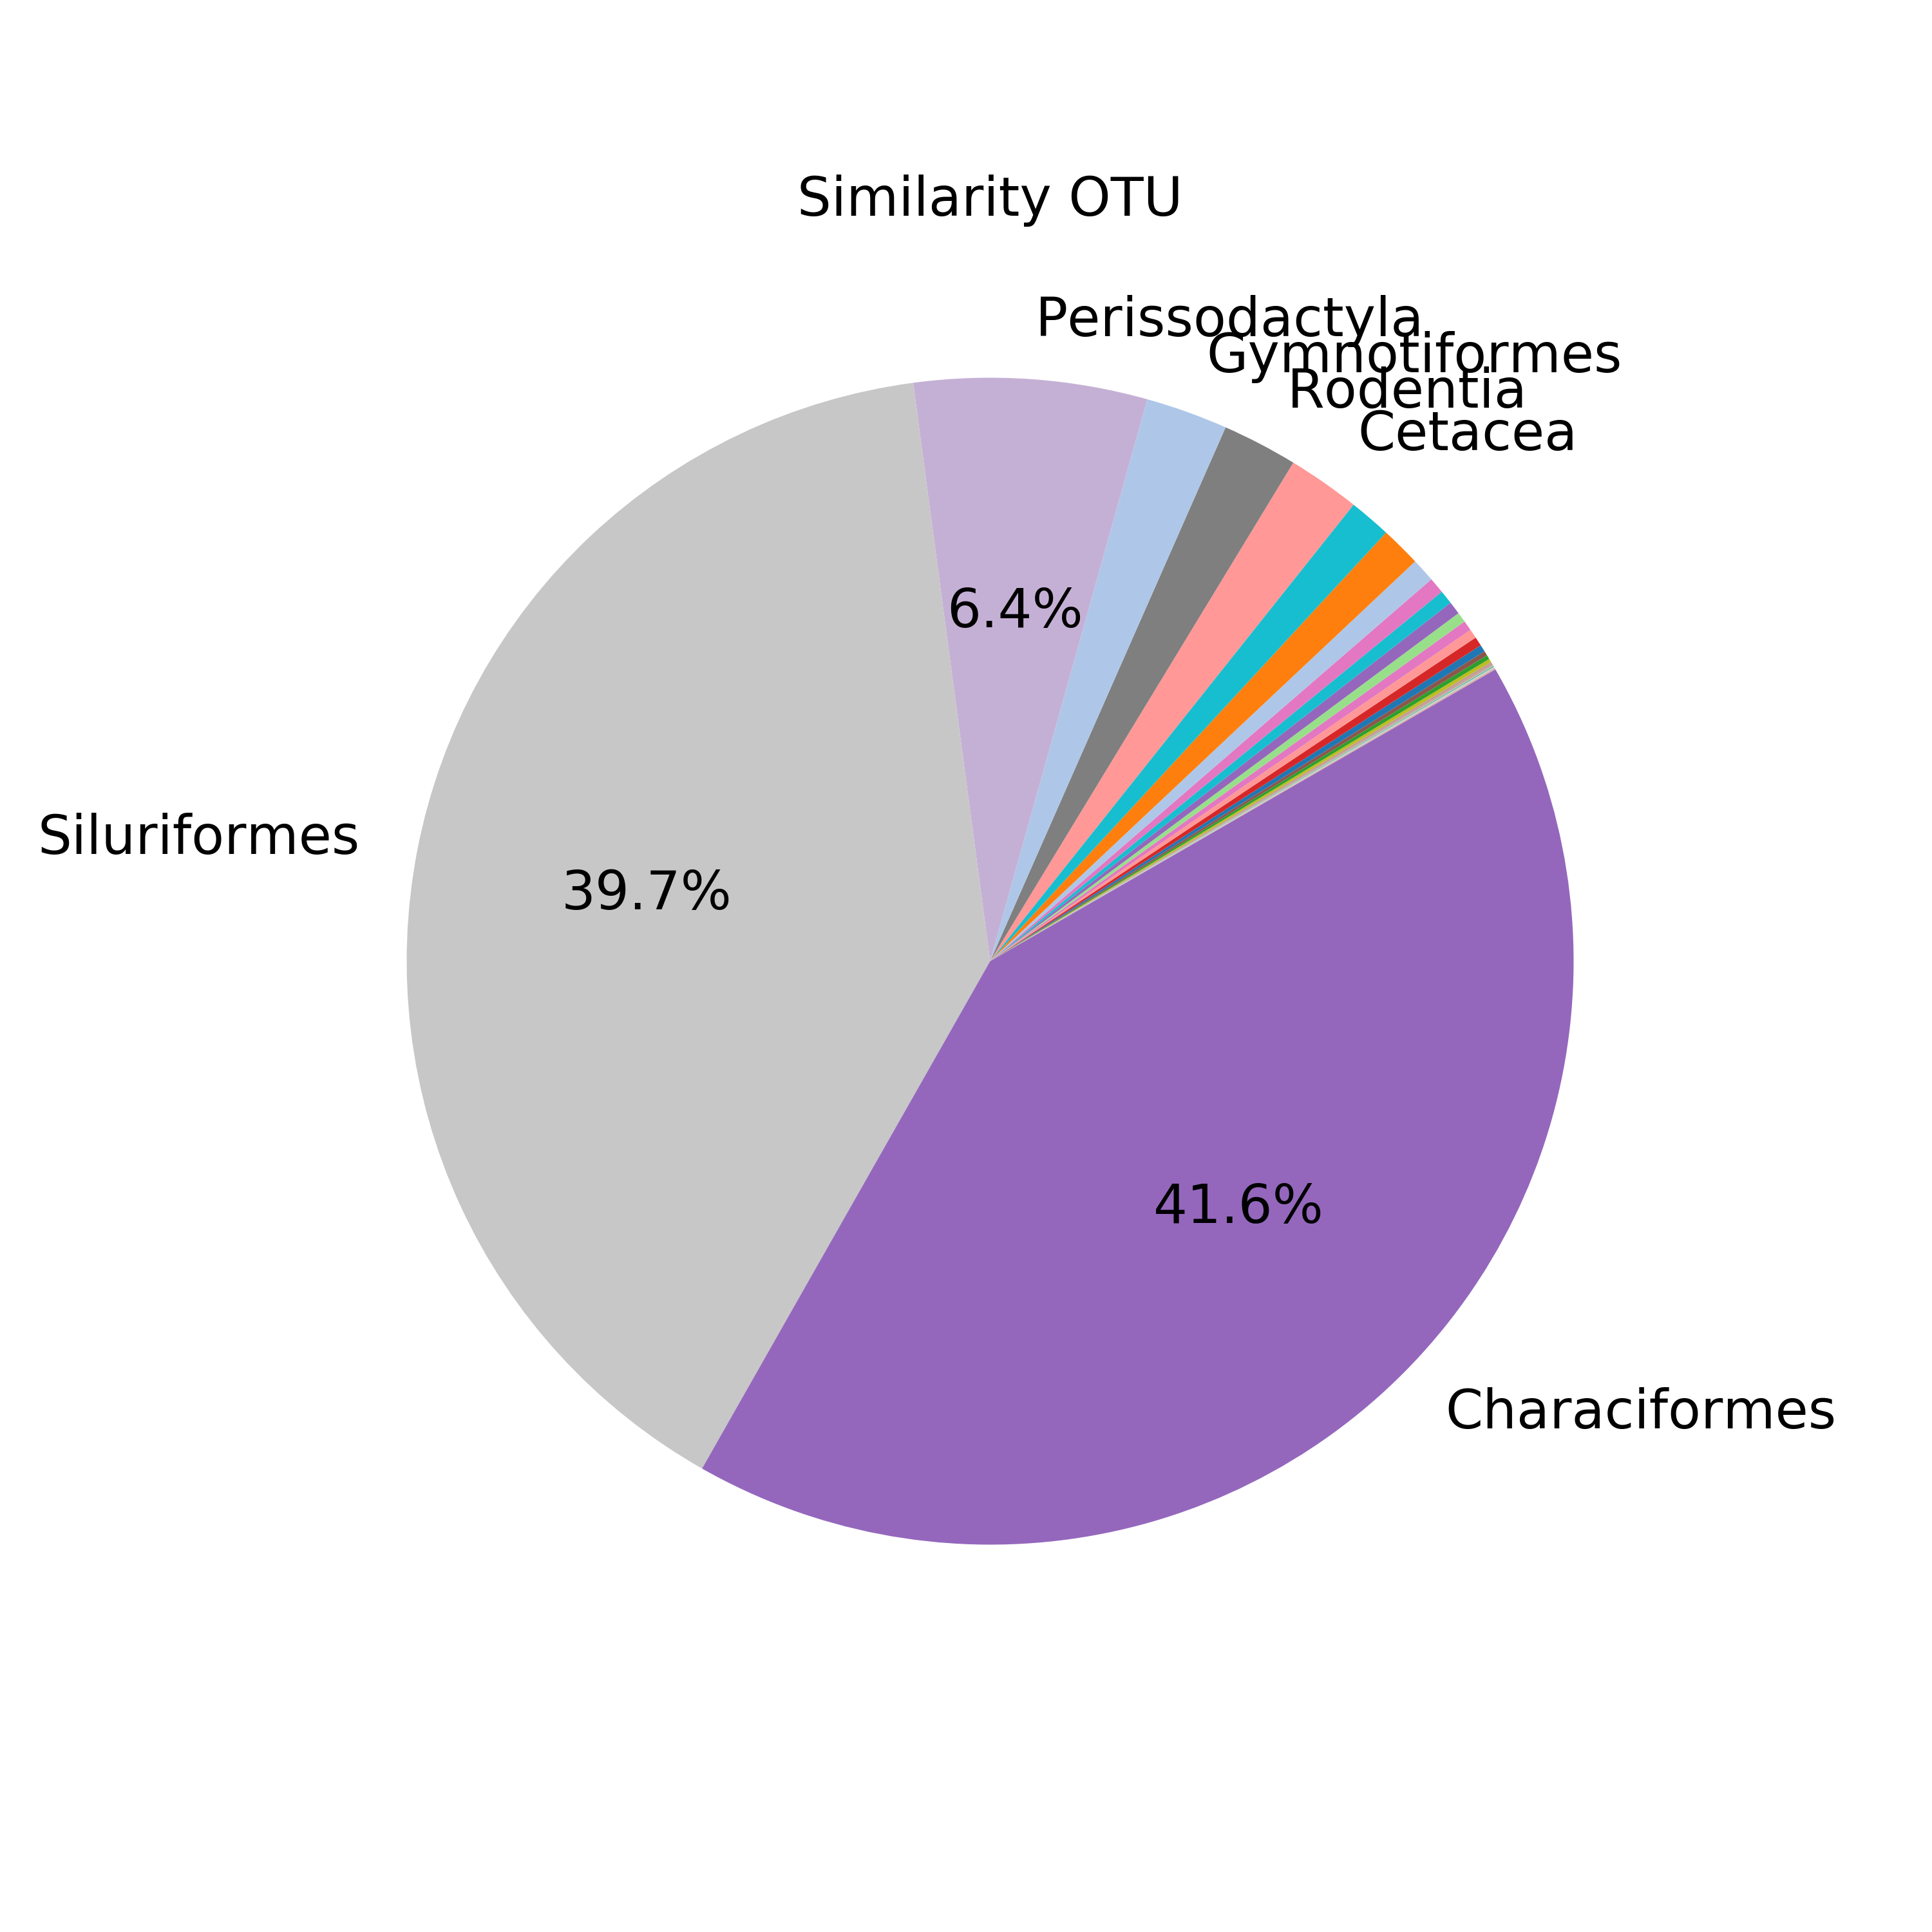
\includegraphics[width=\textwidth]{rfr_sim_sum_pieOTU}
		\caption{}
		\label{fig:simotusum}
	\end{subfigure}
	\begin{subfigure}{0.45\textwidth}
		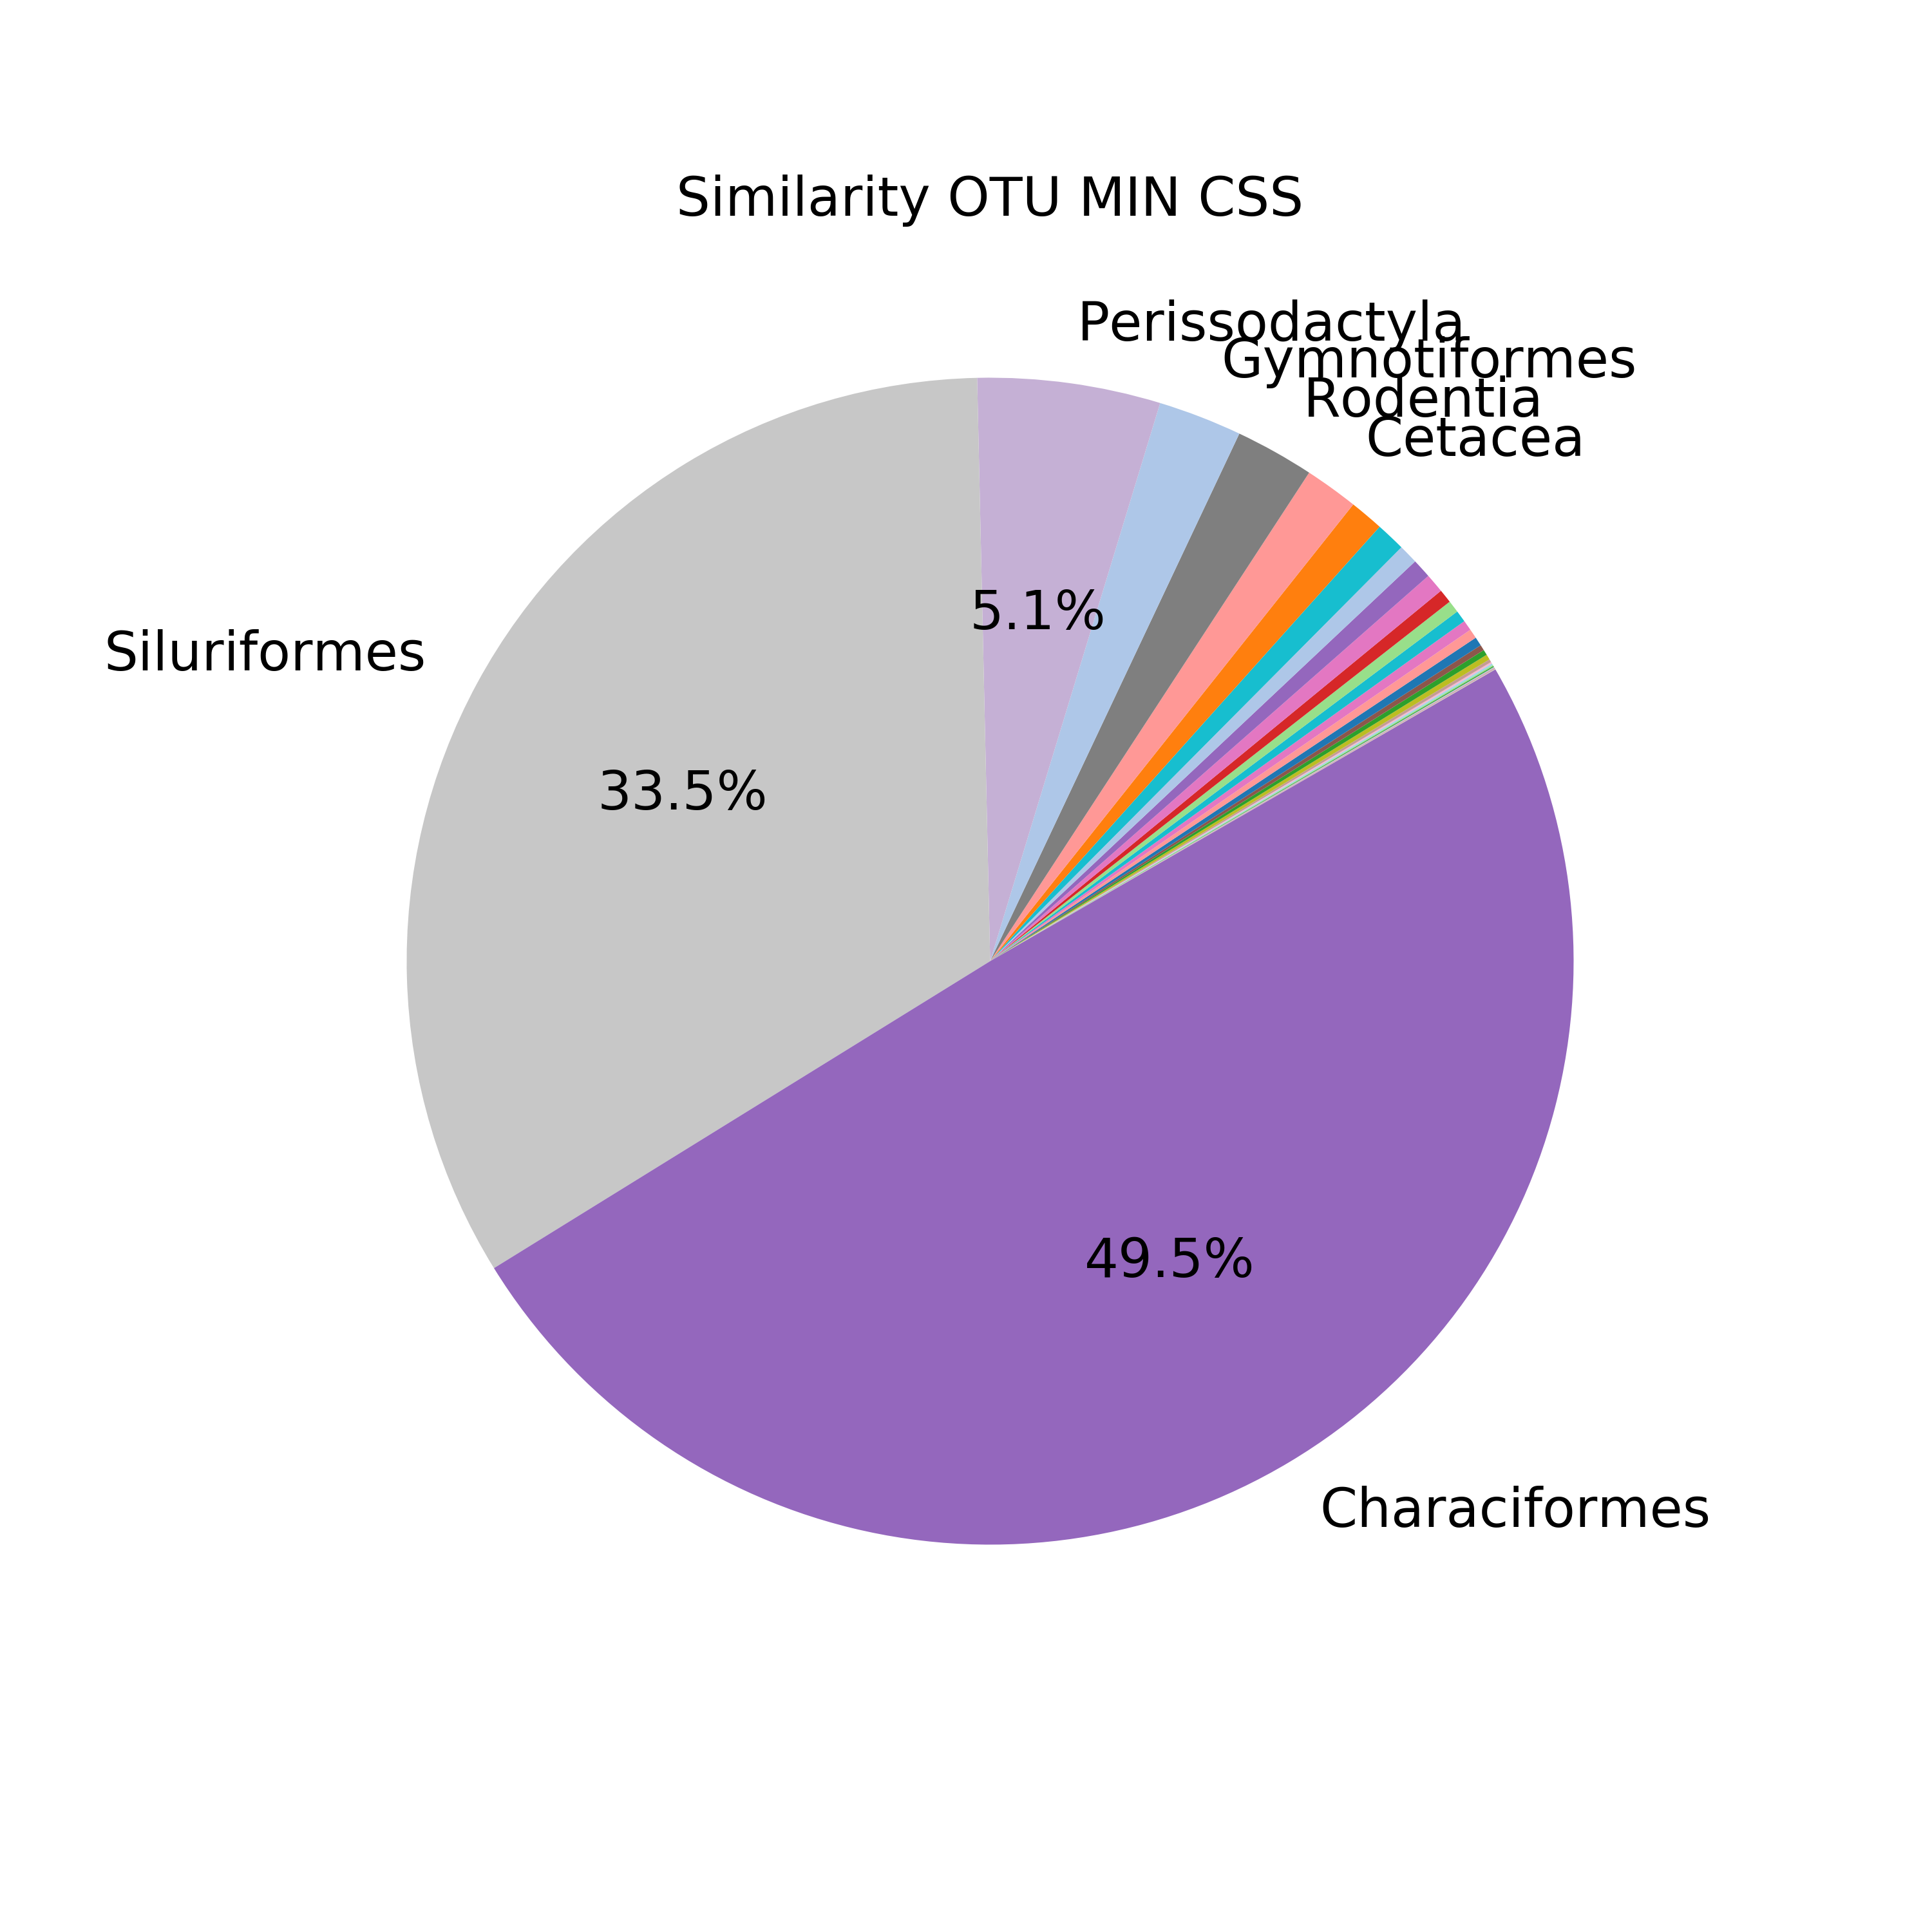
\includegraphics[width=\textwidth]{rfr_sim_sum_pieOTU MIN CSS}
		\caption{}
		\label{fig:simotumincsssum}
	\end{subfigure}
	\caption{Species' importance per taxonomic order as calculated by Random Forest in the maximum similarity test. Averaging the importance for the sets: OTU \ref{fig:simotumean}, and OTU MIN CSS \ref{fig:simotumincssmean}. Summing the importance for the sets: OTU \ref{fig:simotusum}, and OTU MIN CSS \ref{fig:simotumincsssum}.  }
	\label{fig:simpieappendix}
\end{figure}

\begin{figure}[h]
	\centering
	\begin{subfigure}{0.45\textwidth}
		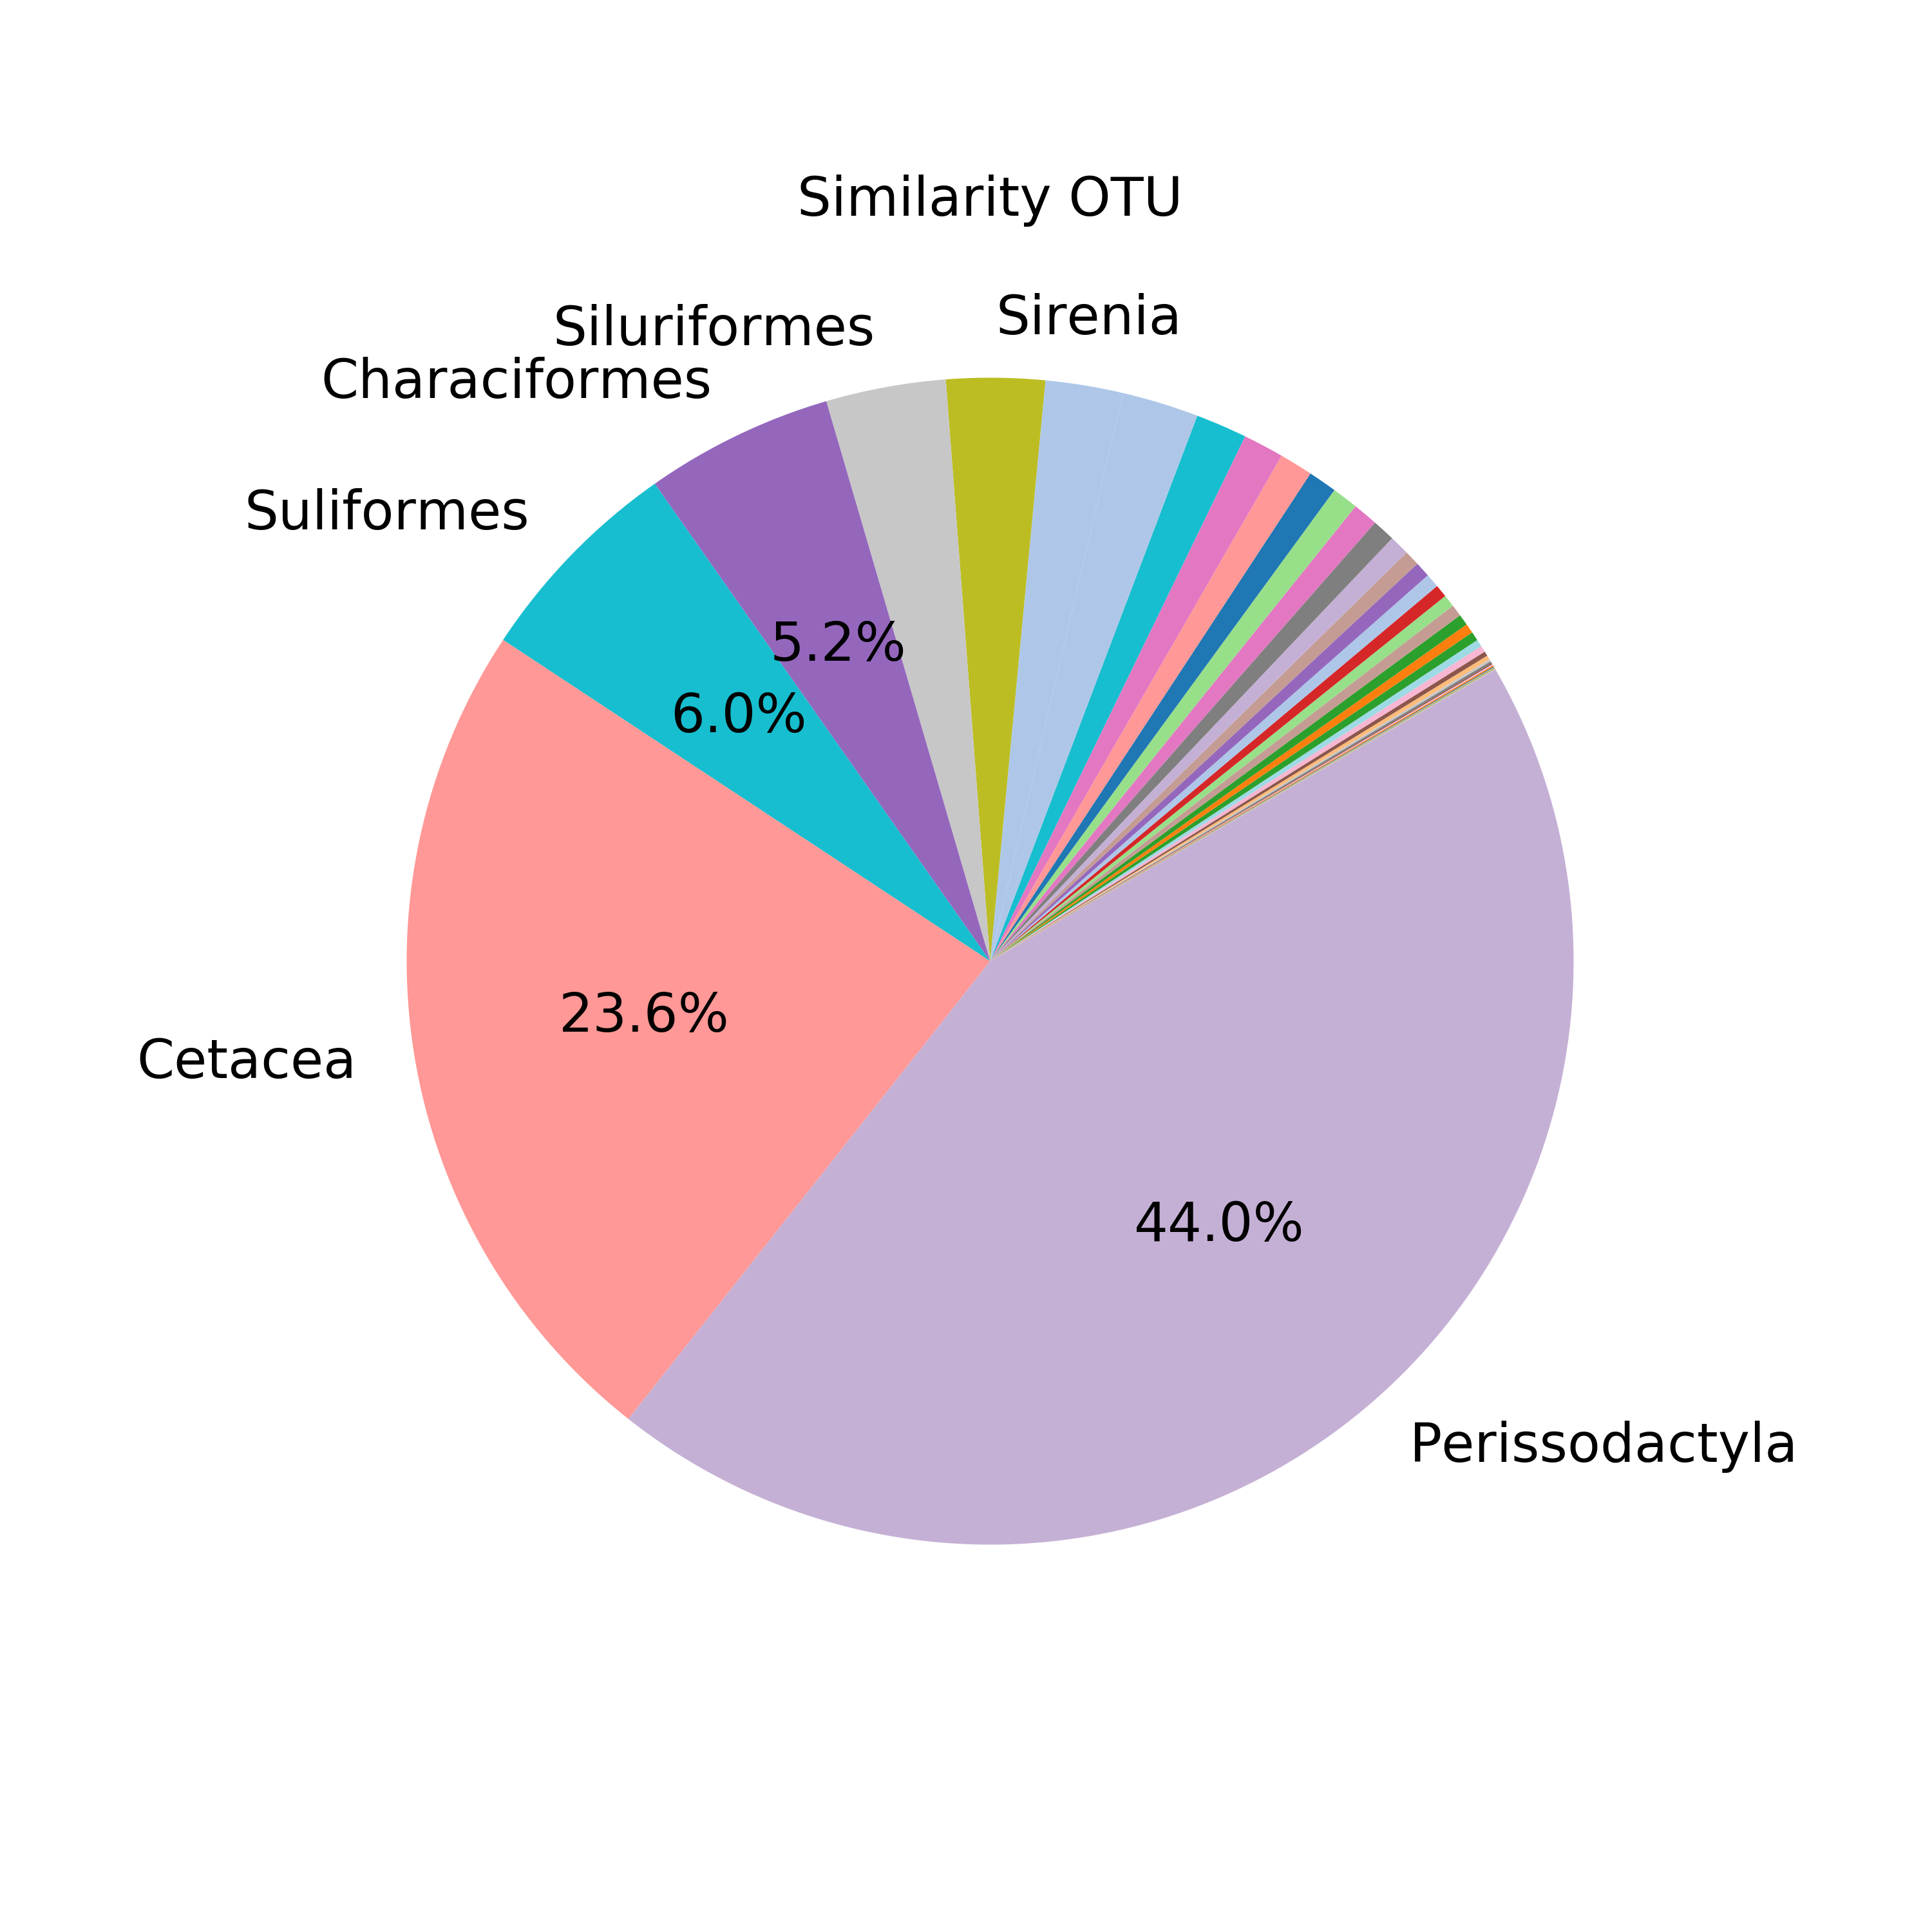
\includegraphics[width=\textwidth]{rfr_dis_mean_pieOTU}
		\caption{}
		\label{fig:dissimotumean}
	\end{subfigure}	
	\begin{subfigure}{0.45\textwidth}
		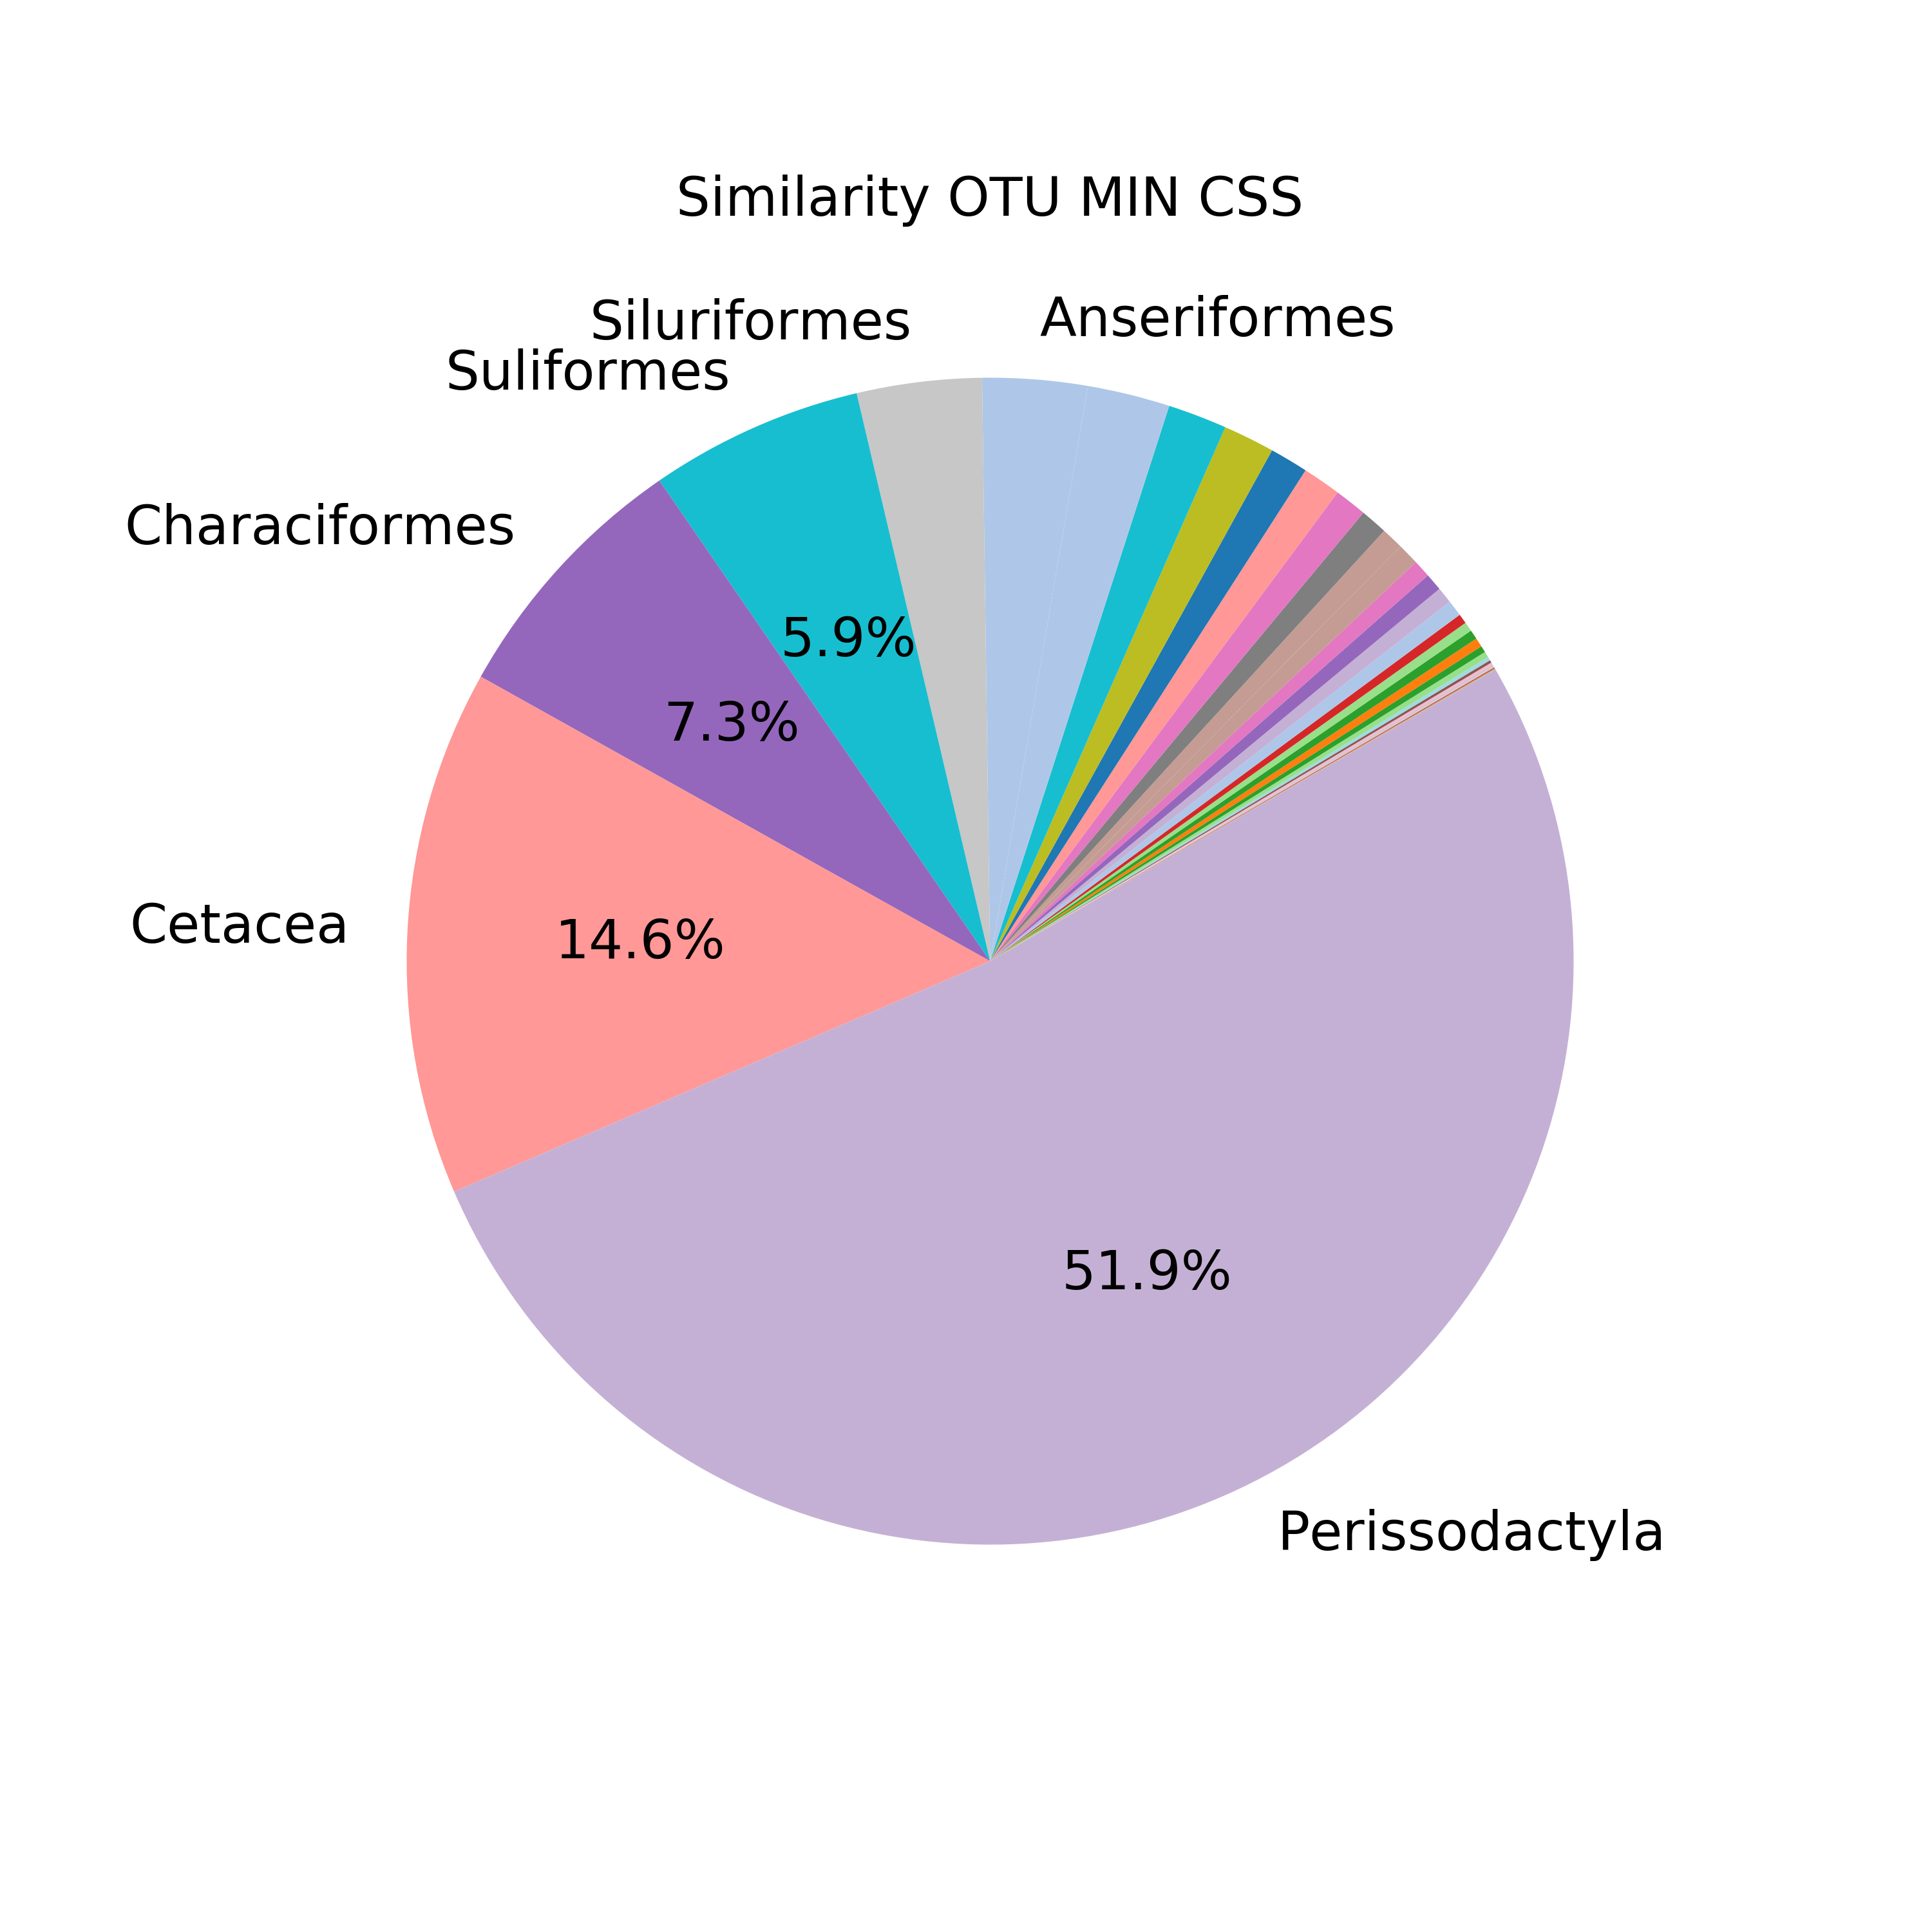
\includegraphics[width=\textwidth]{rfr_dis_mean_pieOTU MIN CSS}
		\caption{}
		\label{fig:dissimotumincssmean}
	\end{subfigure}\\
	\begin{subfigure}{0.45\textwidth}
	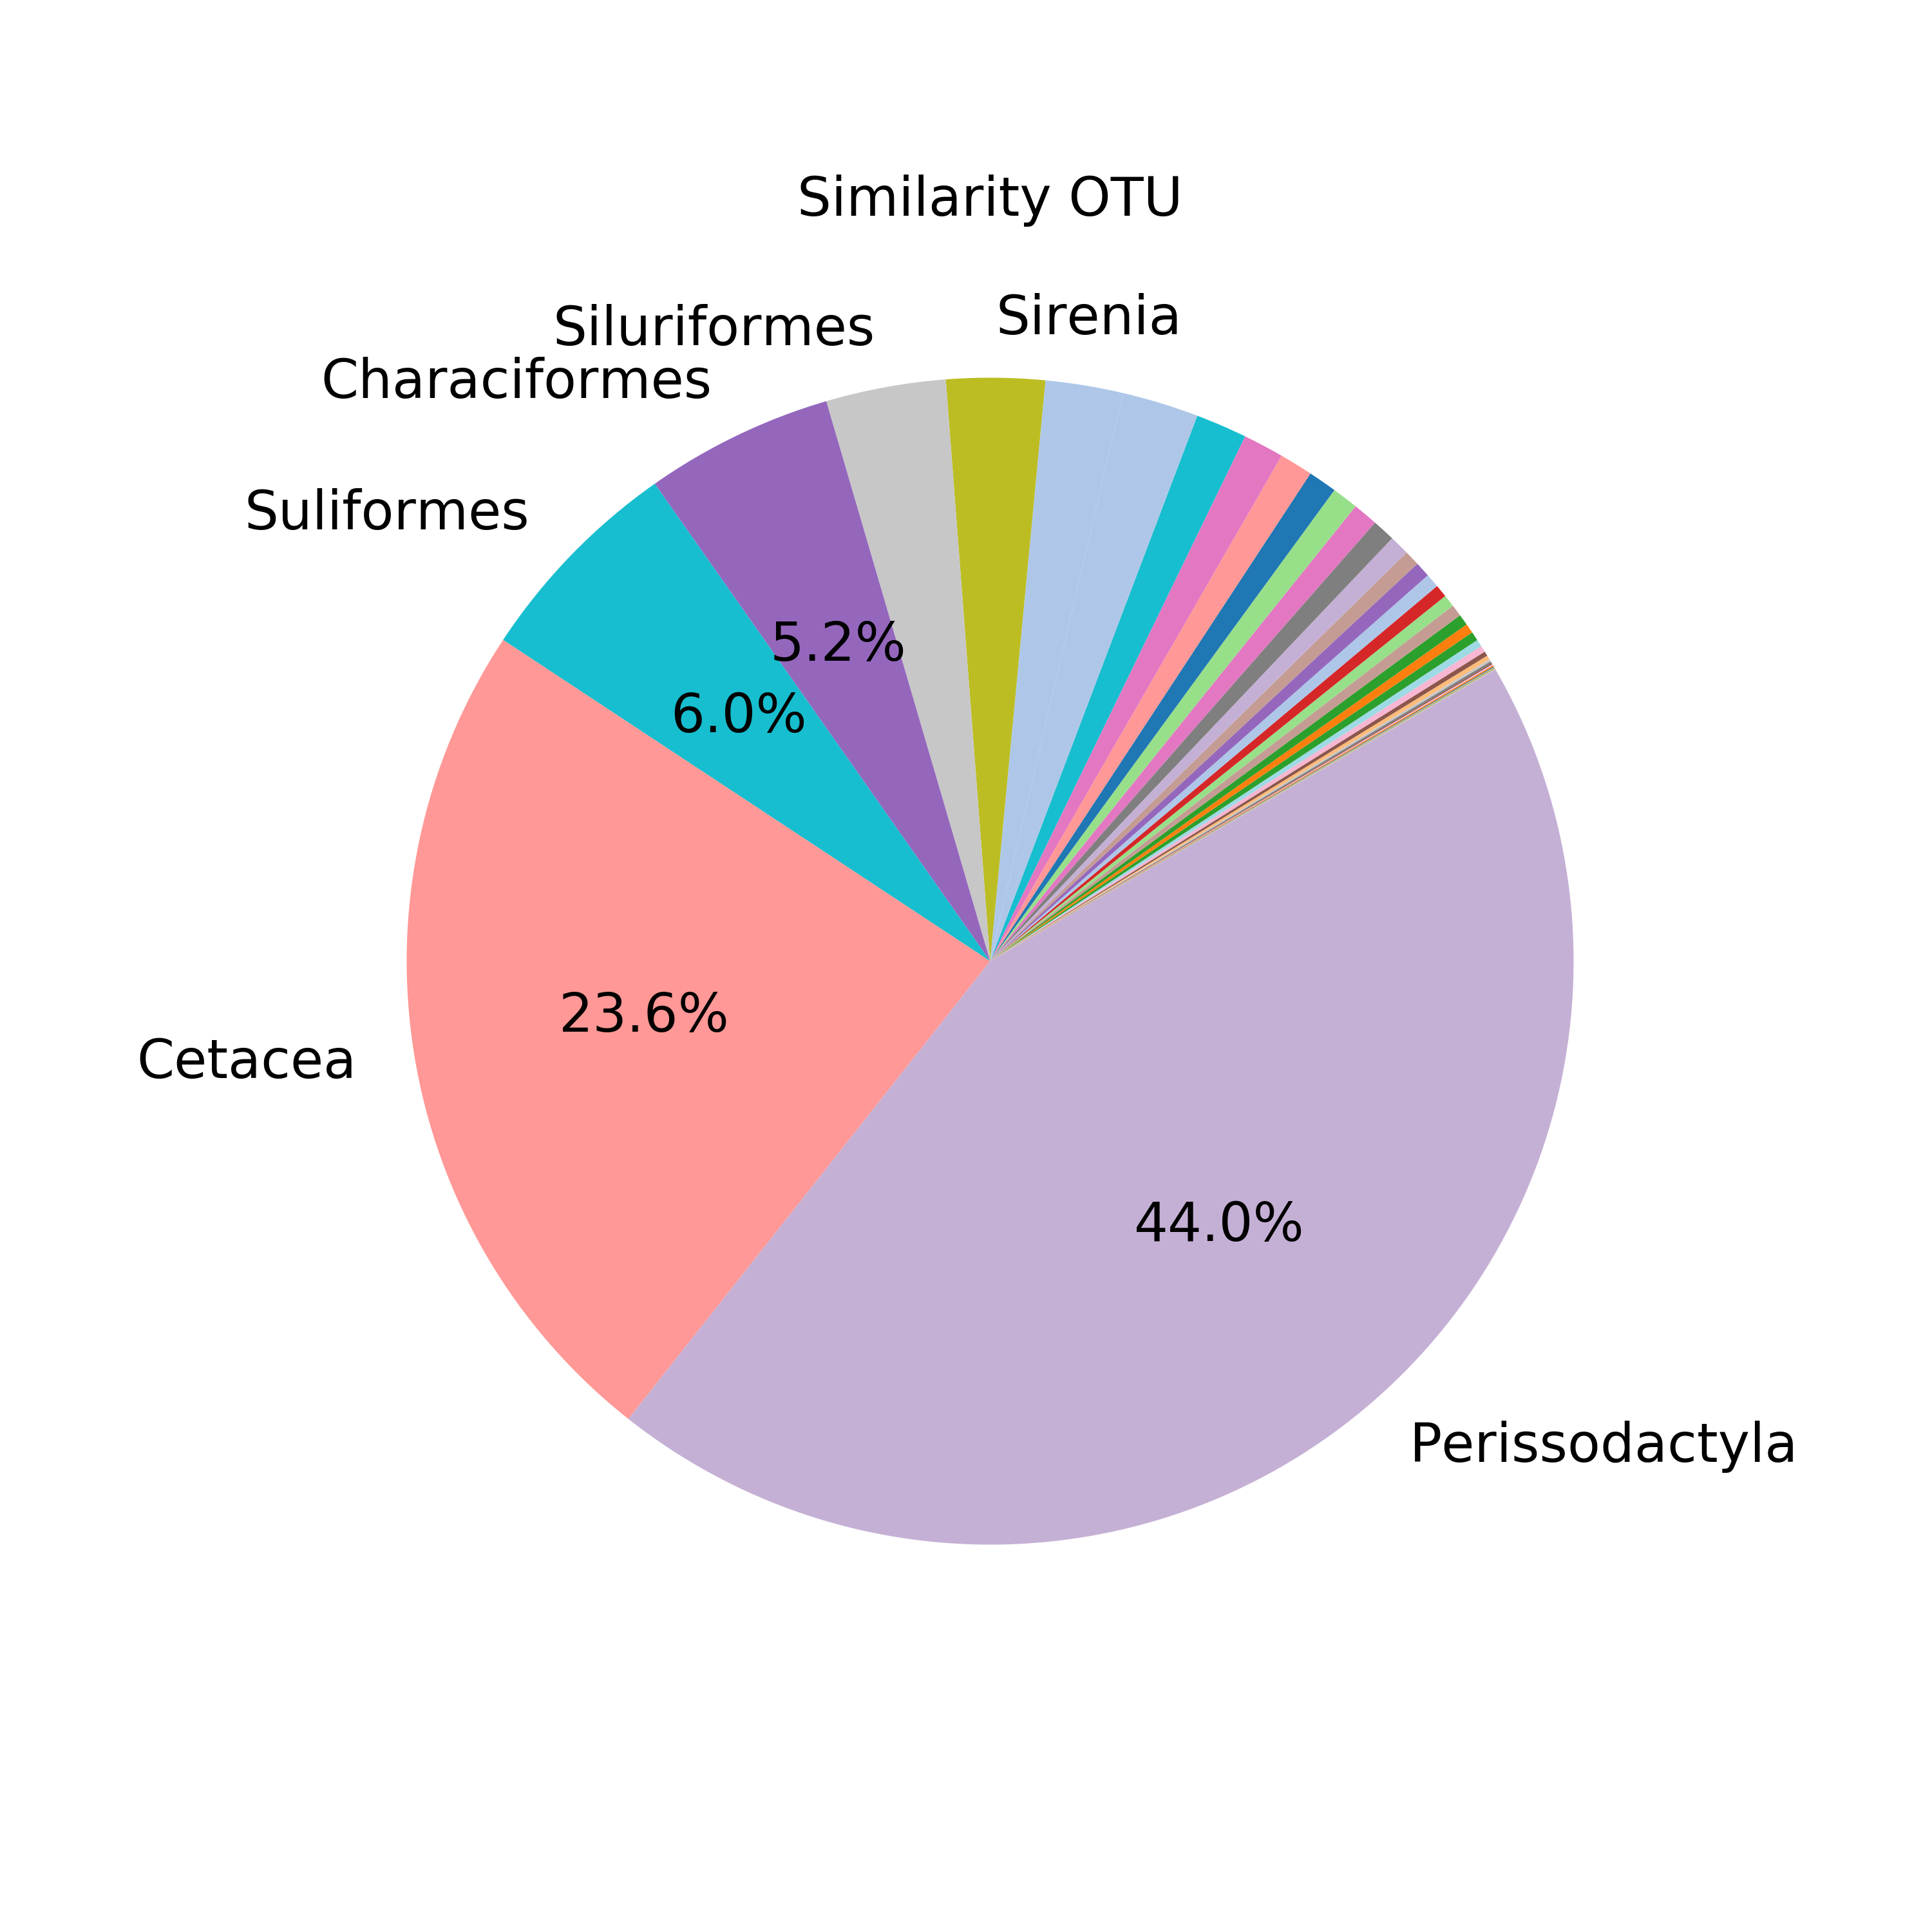
\includegraphics[width=\textwidth]{rfr_dis_sum_pieOTU}
	\caption{}
	\label{fig:dissimotusum}
\end{subfigure}	
\begin{subfigure}{0.45\textwidth}
	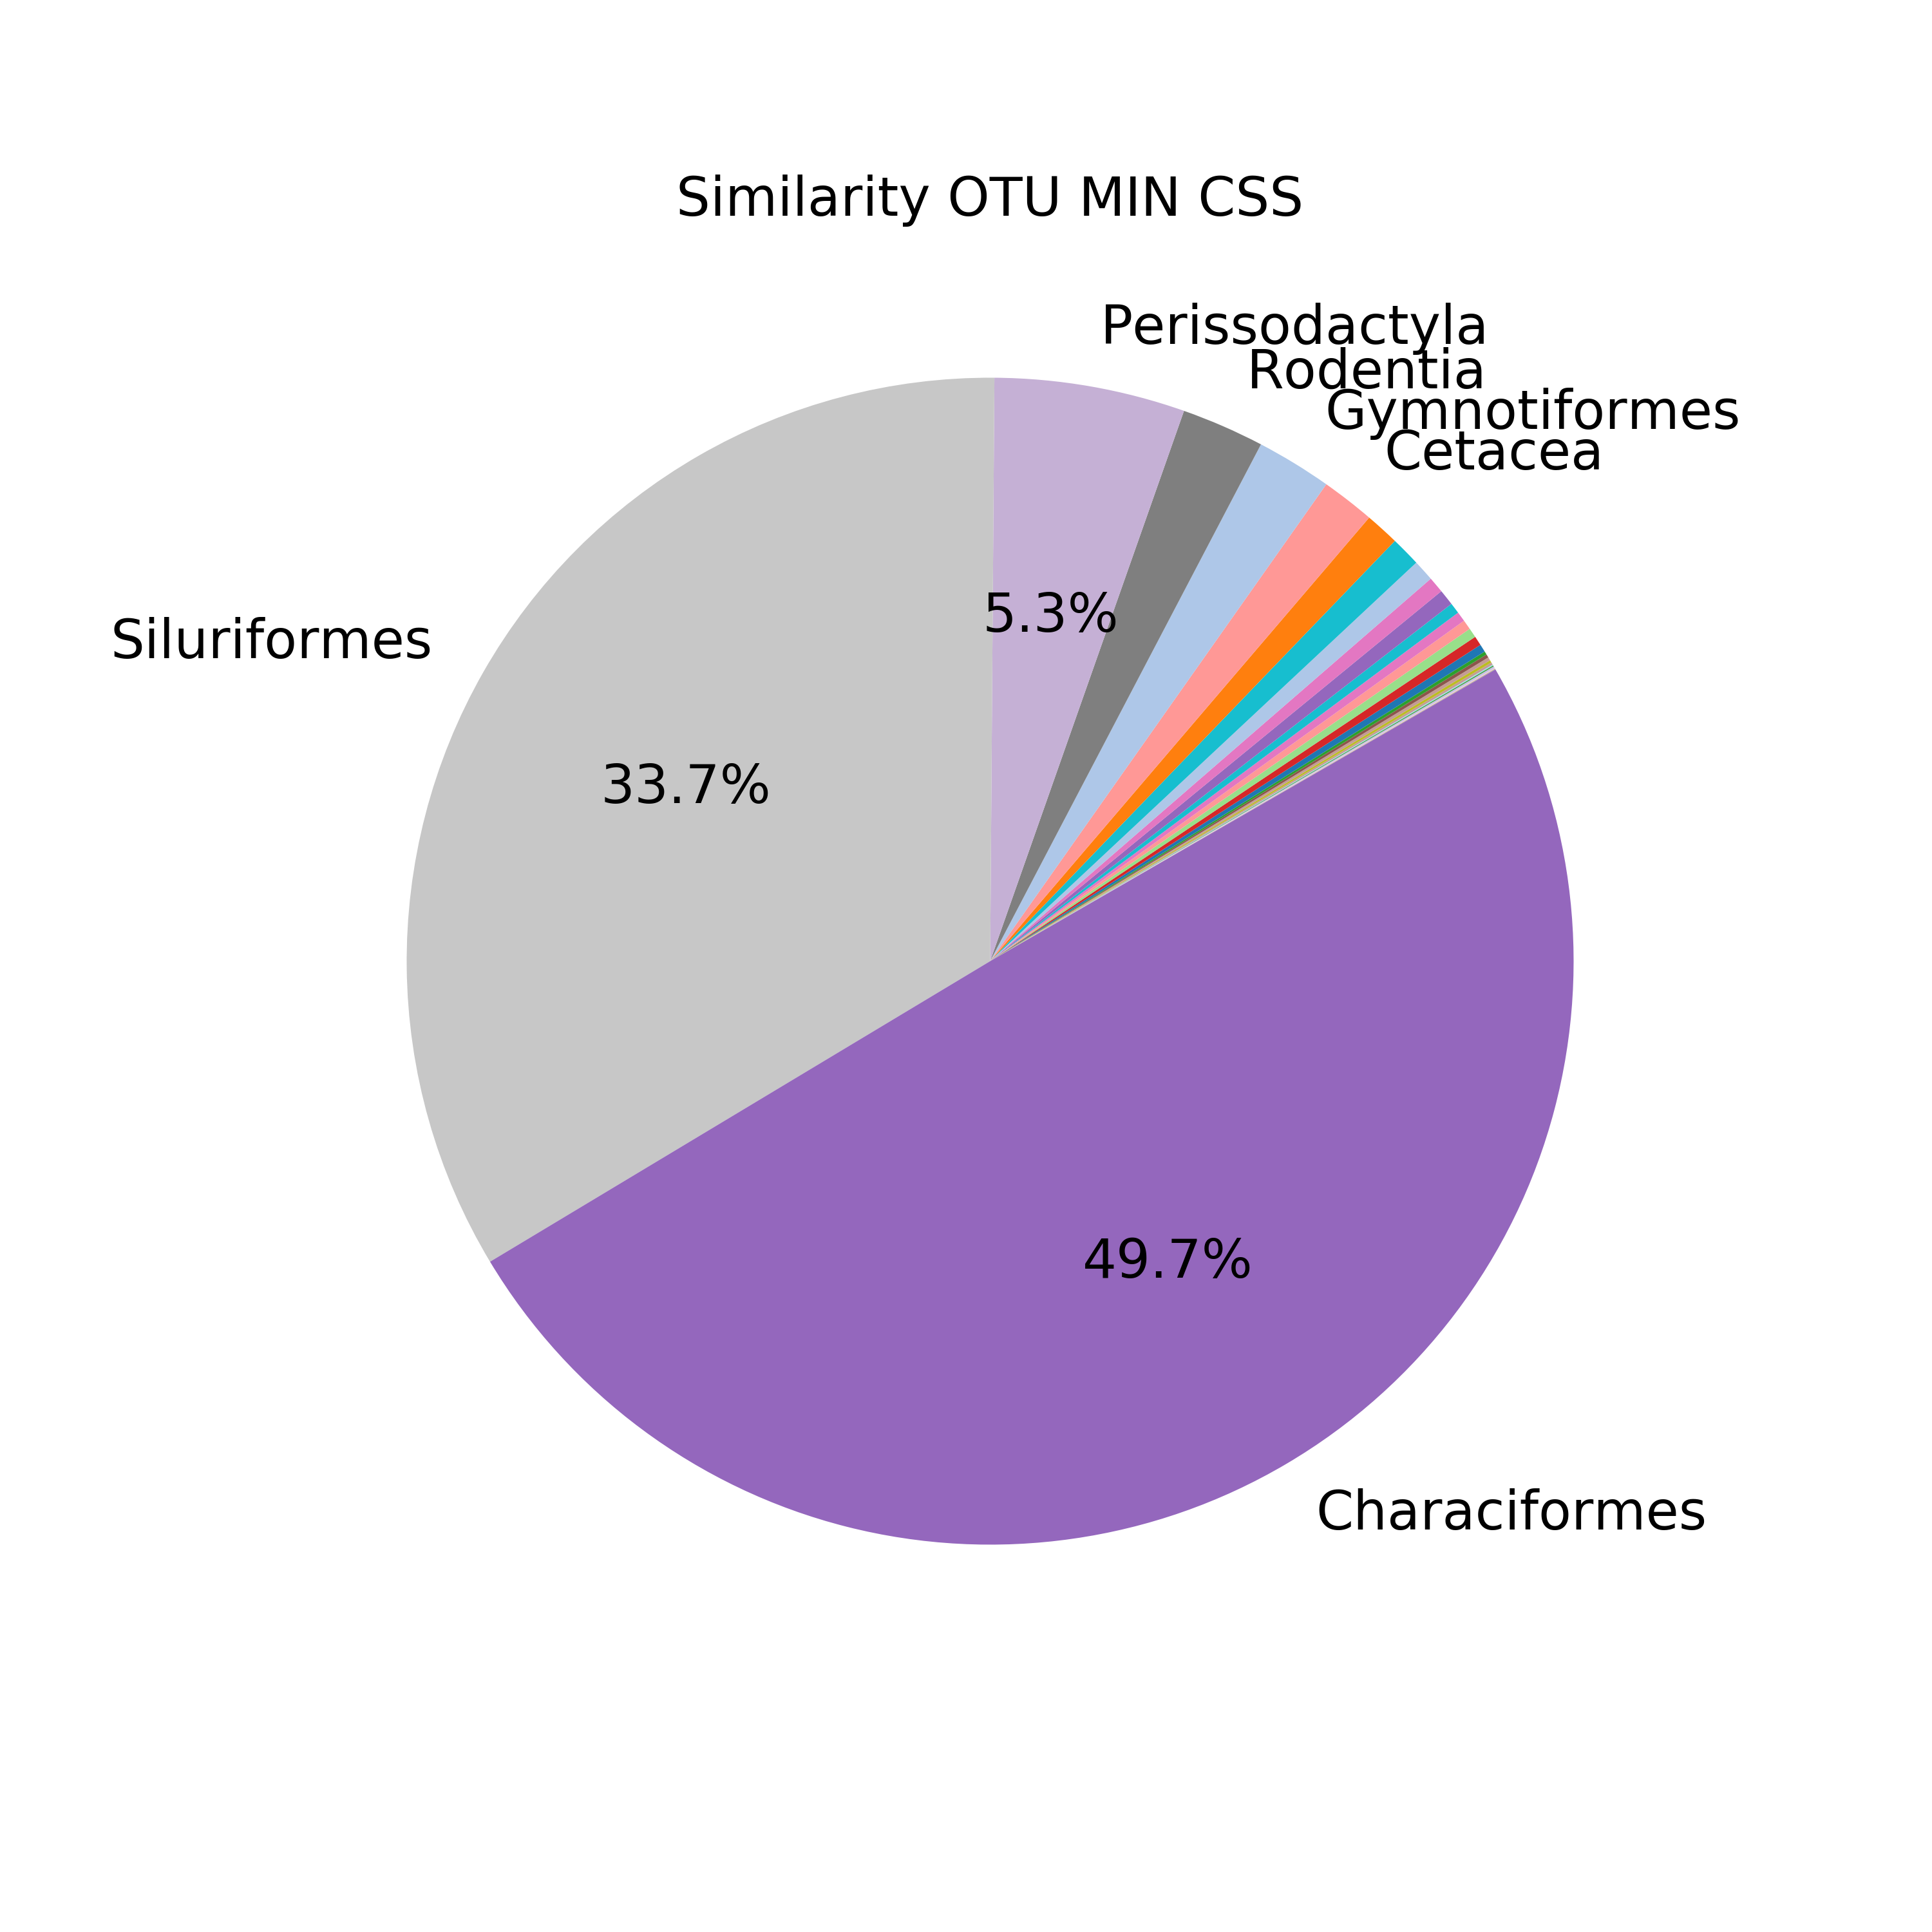
\includegraphics[width=\textwidth]{rfr_dis_sum_pieOTU MIN CSS}
	\caption{}
	\label{fig:dissimotumincsssum}
\end{subfigure}
	\caption{Species' importance per taxonomic order as calculated by Random Forest in the maximum similarity test. Averaging the importance for the sets: OTU \ref{fig:dissimotumean}, and OTU MIN CSS \ref{fig:dissimotumincssmean}. Summing the importance for the sets: OTU \ref{fig:dissimotusum}, and OTU MIN CSS \ref{fig:dissimotumincsssum}. }
	\label{fig:dispieappendix}
\end{figure}
%
%\subsubsection*{Debian/Ubuntu:}
%\begin{verbatim} 
%sudo apt-get install texlive texlive-latex-extra 
%sudo apt-get install psutils
%\end{verbatim}
